\documentclass[11pt]{article}
\usepackage[margin=18mm,headheight=22pt]{geometry}
\usepackage{amsmath}
\usepackage{fontspec}
\usepackage{unicode-math}
\setmainfont{NewCM10}[Extension=.otf,UprightFont=*-Book,BoldFont=*-Bold,ItalicFont=*-BookItalic,BoldItalicFont=*-BoldItalic]
\setsansfont{NewCMSans10}[Extension=.otf,UprightFont=*-Book,BoldFont=*-Bold,ItalicFont=*-BookOblique,BoldItalicFont=*-BoldOblique]
\setmathfont{NewCMMath-Book.otf}
\usepackage{xcolor}
\definecolor{FAUblue}{HTML}{04316A}
\definecolor{Paperblue}{HTML}{EEF2F7}
\definecolor{EEIgold}{HTML}{CC9C42}
\usepackage{etoolbox,enumitem,booktabs,tabularx,array,needspace,microtype}
\usepackage[most]{tcolorbox}
\usepackage{titlesec,fancyhdr}
\usepackage[hidelinks]{hyperref}
\usepackage{draftwatermark}
\SetWatermarkText{Made by Thanate Amornjiraporn (Focus)}
\SetWatermarkColor{black!7}\SetWatermarkFontSize{30pt}\SetWatermarkAngle{45}
\setlength{\parindent}{0pt}
\setlength{\parskip}{5pt}
\setlist{itemsep=2pt,topsep=3pt,leftmargin=1.6em,beginpenalty=10000,endpenalty=10000}
\raggedbottom
\clubpenalty=10000 \widowpenalty=10000 \displaywidowpenalty=10000 \interlinepenalty=10000
\setcounter{secnumdepth}{0}
\setcounter{tocdepth}{1}
\pagestyle{fancy}\fancyhf{}
\fancyhead[L]{\small\sffamily\color{FAUblue} From Fundamentals to AI Apocalypse · EEI · Appendix A}
\fancyhead[R]{\small\sffamily Appendix A: Coordinate systems}
\fancyfoot[C]{\small\thepage}
\titleformat{\section}{\Large\bfseries\sffamily\color{FAUblue}}{}{0pt}{}
\titleformat{\subsection}{\large\bfseries\sffamily\color{FAUblue}}{}{0pt}{}
\titlespacing*{\section}{0pt}{16pt}{6pt}
\preto\section{\Needspace{8\baselineskip}}
\preto\subsection{\Needspace{6\baselineskip}}
\newtcolorbox{equationcard}[1]{colback=Paperblue,colframe=Paperblue,boxrule=0pt,arc=0pt,left=10pt,right=10pt,top=6pt,bottom=6pt,title={#1},fonttitle=\small\bfseries\sffamily,coltitle=FAUblue,before skip=8pt,after skip=8pt}
\newtcolorbox{workedbox}[1]{colback=white,colframe=EEIgold,boxrule=0pt,leftrule=3pt,arc=0pt,left=10pt,top=4pt,bottom=4pt,title={#1},fonttitle=\small\bfseries\sffamily,coltitle=FAUblue,attach title to upper={\par},before skip=8pt,after skip=8pt}
\newtcolorbox{recallbox}[1]{colback=white,colframe=FAUblue,boxrule=0pt,leftrule=3pt,arc=0pt,left=10pt,top=4pt,bottom=4pt,title={#1},fonttitle=\small\bfseries\sffamily,coltitle=FAUblue,attach title to upper={\par},before skip=8pt,after skip=8pt}
\usepackage{environ}
\newsavebox\measurebox
% Typeset the section once invisibly to measure it; start a new page if it will not fit in what is left.
\makeatletter
\newif\ifkeep@measuring
\NewEnviron{keepsection}{%
  \ifkeep@measuring \BODY \else
    \edef\keep@sec{\the\value{section}}\edef\keep@sub{\the\value{subsection}}%
    \setbox\measurebox\vbox{\hsize\linewidth\keep@measuringtrue\def\Needspace##1{}\BODY}%
    \setcounter{section}{\keep@sec}\setcounter{subsection}{\keep@sub}%
    \dimen2=\ht\measurebox \advance\dimen2\dp\measurebox
    \dimen@=\textheight
    \ifdim\pagegoal<\maxdimen
      \dimen@=\pagegoal \advance\dimen@-\pagetotal
      \ifdim\dimen2>\dimen@ \clearpage \dimen@=\textheight \fi
    \fi
    % if it fits, nothing inside may force an early break
    \ifdim\dimen2>\dimen@ \BODY \else \begingroup\def\Needspace##1{}\BODY\endgroup \fi
  \fi}
\makeatother
\newtcolorbox{notebox}{colback=Paperblue,colframe=Paperblue,boxrule=0pt,arc=0pt,left=8pt,right=8pt,top=4pt,bottom=4pt,before skip=6pt,after skip=6pt}
\newtcolorbox{plainbox}{colback=white,colframe=FAUblue,boxrule=0pt,leftrule=3pt,arc=0pt,left=10pt,right=8pt,top=4pt,bottom=4pt,before skip=6pt,after skip=8pt}
\usetikzlibrary{arrows.meta}
\title{\sffamily\bfseries\color{FAUblue}Appendix A: Coordinate systems}
\author{Electrical Engineering I \ensuremath{\cdot} Module 92315 \ensuremath{\cdot} Appendix A\\[2pt]\small From Fundamentals to AI Apocalypse · personal study guide}
\date{}
\begin{document}
\maketitle
\begingroup\footnotesize\setlength{\parskip}{0pt}\tableofcontents\endgroup
\clearpage

\Needspace{9\baselineskip}
{\large A reference for Cartesian, cylindrical and spherical coordinates: how each describes a point, its unit vectors, how to convert between them, and the path, area and volume elements that every field integral in the course is built from. Keep it open next to the exercises.}


\begin{keepsection}
\Needspace{16\baselineskip}
\section{A.1 Three ways to locate a point}

\Needspace{13\baselineskip}
Each system gives a point three numbers. \textbf{Cartesian} coordinates measure along three fixed directions. \textbf{Cylindrical} coordinates give the distance \textit{ρ} from the \textit{z}-axis, the angle \textit{φ} around it (measured from the \textit{x}-axis) and the height \textit{z}. \textbf{Spherical} coordinates give the distance \textit{r} from the origin, the angle \textit{ϑ} down from the \textit{z}-axis and the same angle \textit{φ}.

\Needspace{10\baselineskip}
\begin{center}\small\begin{tabularx}{\linewidth}{>{\raggedright\arraybackslash}X>{\raggedright\arraybackslash}X>{\raggedright\arraybackslash}X}\toprule
\textbf{System} & \textbf{Coordinates and ranges} & \textbf{Unit vectors} \\ \midrule
Cartesian & \textit{x}, \textit{y}, \textit{z}, each from \ensuremath{-}\ensuremath{\infty} to \ensuremath{\infty} & \textit{e}\textsubscript{x}, \textit{e}\textsubscript{y}, \textit{e}\textsubscript{z} \\
Cylindrical & 0 \ensuremath{\leq} \textit{ρ} \ensuremath{<} \ensuremath{\infty}, 0 \ensuremath{\leq} \textit{φ} \ensuremath{<} 2π, \textit{z} from \ensuremath{-}\ensuremath{\infty} to \ensuremath{\infty} & \textit{e}\textsubscript{ρ}, \textit{e}\textsubscript{φ}, \textit{e}\textsubscript{z} \\
Spherical & 0 \ensuremath{\leq} \textit{r} \ensuremath{<} \ensuremath{\infty}, 0 \ensuremath{\leq} \textit{ϑ} \ensuremath{\leq} π, 0 \ensuremath{\leq} \textit{φ} \ensuremath{<} 2π & \textit{e}\textsubscript{r}, \textit{e}\textsubscript{ϑ}, \textit{e}\textsubscript{φ} \\
\bottomrule\end{tabularx}\end{center}

\begin{equationcard}{Cylindrical to Cartesian}
\[ \begin{gathered} {x}\, =\, {ρ}\, \cos \, {φ} \\ {y}\, =\, {ρ}\, \sin \, {φ} \\ {z}\, =\, {z} \end{gathered} \]
{\small \emph{Read it as: “x is rho cos phi, y is rho sin phi, and z stays z”.}\par Going back: \textit{ρ} = \ensuremath{\sqrt{{x}^{2}\, +\, {y}^{2}}}, and \textit{φ} from tan \textit{φ} = \textit{y}/\textit{x}, choosing the quadrant from the signs of \textit{x} and \textit{y}.}
\end{equationcard}

\begin{equationcard}{Spherical to Cartesian}
\[ \begin{gathered} {x}\, =\, {r}\, \sin \, {ϑ}\, \cos \, {φ} \\ {y}\, =\, {r}\, \sin \, {ϑ}\, \sin \, {φ} \\ {z}\, =\, {r}\, \cos \, {ϑ} \end{gathered} \]
{\small \emph{Read it as: “x is r sin theta cos phi, y is r sin theta sin phi, z is r cos theta”.}\par \textit{r} sin \textit{ϑ} is the point’s distance from the \textit{z}-axis, so it plays the part of \textit{ρ}. Going back: \textit{r} = \ensuremath{\sqrt{{x}^{2}\, +\, {y}^{2}\, +\, {z}^{2}}}, cos \textit{ϑ} = \textit{z}/\textit{r}, and \textit{φ} as for cylindrical coordinates.}
\end{equationcard}
\end{keepsection}

\begin{keepsection}
\Needspace{11\baselineskip}
\section{A.2 Unit vectors and cross products}

\Needspace{8\baselineskip}
In every system the three unit vectors are perpendicular to each other and have length 1, so a dot product of two different ones is 0. They form a right-handed set in the order listed: crossing one with the next gives the third, and the order runs round in a circle. Crossing in the opposite order flips the sign.

\Needspace{11\baselineskip}
Only the Cartesian unit vectors are the same everywhere. \textit{e}\textsubscript{ρ}, \textit{e}\textsubscript{φ}, \textit{e}\textsubscript{r} and \textit{e}\textsubscript{ϑ} change direction from point to point, which matters as soon as you add or integrate vectors (A.6).

\Needspace{14\baselineskip}
\begin{center}
\begin{minipage}[t]{0.465\linewidth}\centering
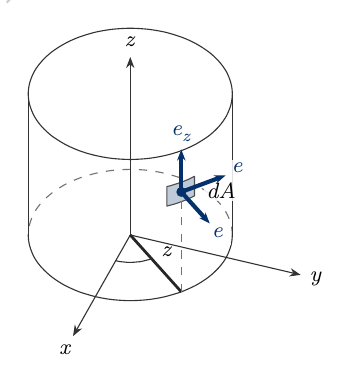
\begin{tikzpicture}[line join=round]
\draw[black!55,dashed] plot[smooth,tension=0.5] coordinates {(2.700,-2.734) (2.695,-2.662) (2.680,-2.590) (2.655,-2.518) (2.623,-2.450) (2.579,-2.381) (2.527,-2.318) (2.466,-2.257) (2.398,-2.200) (2.320,-2.146) (2.237,-2.095) (2.147,-2.052) (2.052,-2.012) (1.951,-1.980) (1.847,-1.951) (1.739,-1.930) (1.629,-1.913) (1.517,-1.904) (1.404,-1.901) (1.291,-1.904) (1.179,-1.913) (1.069,-1.930) (0.961,-1.951) (0.857,-1.980) (0.756,-2.012) (0.661,-2.052) (0.571,-2.095) (0.488,-2.146) (0.410,-2.200) (0.342,-2.257) (0.281,-2.318) (0.229,-2.381) (0.185,-2.450) (0.153,-2.518) (0.128,-2.590) (0.113,-2.662) (0.108,-2.734)};
\draw[black!80] plot[smooth,tension=0.5] coordinates {(0.108,-2.734) (0.113,-2.806) (0.128,-2.878) (0.153,-2.950) (0.185,-3.019) (0.229,-3.087) (0.281,-3.150) (0.342,-3.211) (0.410,-3.269) (0.488,-3.323) (0.571,-3.373) (0.661,-3.416) (0.756,-3.456) (0.857,-3.488) (0.961,-3.517) (1.069,-3.539) (1.179,-3.555) (1.291,-3.564) (1.404,-3.568) (1.517,-3.564) (1.629,-3.555) (1.739,-3.539) (1.847,-3.517) (1.951,-3.488) (2.052,-3.456) (2.147,-3.416) (2.237,-3.373) (2.320,-3.323) (2.398,-3.269) (2.466,-3.211) (2.527,-3.150) (2.579,-3.087) (2.623,-3.019) (2.655,-2.950) (2.680,-2.878) (2.695,-2.806) (2.700,-2.734)};
\draw[black!80] plot[smooth,tension=0.5] coordinates {(0.961,-1.724) (1.069,-1.746) (1.179,-1.762) (1.291,-1.771) (1.404,-1.775) (1.517,-1.771) (1.629,-1.762) (1.739,-1.746) (1.847,-1.724) (1.951,-1.697) (2.052,-1.663) (2.147,-1.624) (2.237,-1.580) (2.320,-1.530) (2.398,-1.478) (2.466,-1.420) (2.527,-1.359) (2.579,-1.294) (2.623,-1.226) (2.655,-1.157) (2.680,-1.087) (2.695,-1.013) (2.700,-0.941) (2.695,-0.869) (2.680,-0.797) (2.655,-0.725) (2.623,-0.657) (2.579,-0.590) (2.527,-0.526) (2.466,-0.464) (2.398,-0.407) (2.320,-0.353) (2.237,-0.304) (2.147,-0.259) (2.052,-0.220) (1.951,-0.187) (1.847,-0.158) (1.739,-0.137) (1.629,-0.121) (1.517,-0.112) (1.404,-0.108) (1.291,-0.112) (1.179,-0.121) (1.069,-0.137) (0.961,-0.158) (0.857,-0.187) (0.756,-0.220) (0.661,-0.259) (0.571,-0.304) (0.488,-0.353) (0.410,-0.407) (0.342,-0.464) (0.281,-0.526) (0.229,-0.590) (0.185,-0.657) (0.153,-0.725) (0.128,-0.797) (0.113,-0.869) (0.108,-0.941) (0.113,-1.013) (0.128,-1.087) (0.153,-1.157) (0.185,-1.226) (0.229,-1.294) (0.281,-1.359) (0.342,-1.420) (0.410,-1.478) (0.488,-1.530) (0.571,-1.580) (0.661,-1.624) (0.756,-1.663) (0.857,-1.697) (0.961,-1.724)};
\draw[black!80] (2.700,-2.734) -- (2.700,-0.941);
\draw[black!80] (0.108,-2.734) -- (0.108,-0.941);
\draw[-{Stealth[length=4pt]},black!80] (1.404,-2.734) -- (0.677,-4.018);
\node[,inner sep=1pt,font=\footnotesize] at (0.579,-4.190) {\textit{x}};
\draw[-{Stealth[length=4pt]},black!80] (1.404,-2.734) -- (3.569,-3.240);
\node[,inner sep=1pt,font=\footnotesize] at (3.762,-3.285) {\textit{y}};
\draw[-{Stealth[length=4pt]},black!80] (1.404,-2.734) -- (1.404,-0.473);
\node[,inner sep=1pt,font=\footnotesize] at (1.404,-0.275) {\textit{z}};
\filldraw[draw=black!70,fill=FAUblue!25] (1.868,-2.367) -- (1.915,-2.354) -- (1.962,-2.342) -- (2.007,-2.327) -- (2.052,-2.311) -- (2.095,-2.295) -- (2.138,-2.277) -- (2.180,-2.257) -- (2.219,-2.237) -- (2.219,-1.989) -- (2.180,-2.009) -- (2.138,-2.029) -- (2.095,-2.047) -- (2.052,-2.063) -- (2.007,-2.079) -- (1.962,-2.093) -- (1.915,-2.108) -- (1.868,-2.119) -- cycle;
\draw[black!85,line width=1pt] (1.404,-2.734) -- (2.052,-3.456);
\draw[black!55,dashed] (2.052,-3.456) -- (2.052,-2.187);
\draw[black!80] plot[smooth,tension=0.5] coordinates {(1.219,-3.060) (1.256,-3.069) (1.294,-3.074) (1.334,-3.078) (1.373,-3.082) (1.411,-3.082) (1.451,-3.080) (1.490,-3.076) (1.528,-3.073) (1.566,-3.065) (1.604,-3.056) (1.640,-3.047) (1.674,-3.035)};
\node[,inner sep=1pt,font=\footnotesize] at (1.737,-3.374) {\textit{ρ}};
\node[,inner sep=1pt,font=\footnotesize] at (1.471,-3.218) {\textit{φ}};
\node[,inner sep=1pt,font=\footnotesize] at (1.872,-2.948) {\textit{z}};
\node[anchor=west,fill=white,fill opacity=0.85,text opacity=1,inner sep=1pt,font=\footnotesize] at (2.327,-2.169) {\textit{dA}};
\fill[FAUblue] (2.052,-2.187) circle (0.063);
\draw[-{Stealth[length=4pt]},FAUblue,line width=1.5pt] (2.052,-2.187) -- (2.414,-2.588);
\node[text=FAUblue,fill=white,fill opacity=0.85,text opacity=1,inner sep=1pt,font=\footnotesize] at (2.546,-2.735) {\textit{e\textsubscript{ρ}}};
\draw[-{Stealth[length=4pt]},FAUblue,line width=1.5pt] (2.052,-2.187) -- (2.614,-1.978);
\node[text=FAUblue,fill=white,fill opacity=0.85,text opacity=1,inner sep=1pt,font=\footnotesize] at (2.799,-1.909) {\textit{e\textsubscript{φ}}};
\draw[-{Stealth[length=4pt]},FAUblue,line width=1.5pt] (2.052,-2.187) -- (2.052,-1.647);
\node[text=FAUblue,fill=white,fill opacity=0.85,text opacity=1,inner sep=1pt,font=\footnotesize] at (2.052,-1.449) {\textit{e\textsubscript{z}}};
\end{tikzpicture}\par\smallskip{\small\raggedright \textbf{Cylindrical.} P lies on the cylinder of radius \textit{ρ}. Its unit vectors point away from the axis (\textit{e}\textsubscript{ρ}), around it in the direction of growing \textit{φ} (\textit{e}\textsubscript{φ}) and up (\textit{e}\textsubscript{z}). The shaded patch is the wall element d\textit{A}.\par}\end{minipage}\hfill
\begin{minipage}[t]{0.465\linewidth}\centering
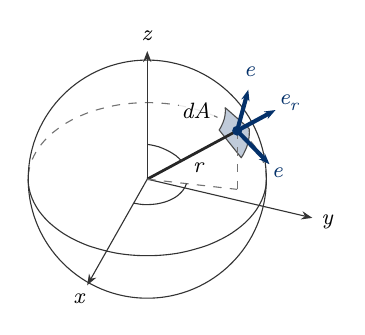
\begin{tikzpicture}[line join=round]
\draw[black!55,dashed] plot[smooth,tension=0.5] coordinates {(3.132,-2.077) (3.127,-1.993) (3.109,-1.908) (3.080,-1.825) (3.040,-1.744) (2.990,-1.667) (2.929,-1.591) (2.858,-1.519) (2.777,-1.453) (2.689,-1.390) (2.592,-1.332) (2.488,-1.282) (2.376,-1.235) (2.259,-1.197) (2.137,-1.165) (2.011,-1.138) (1.883,-1.120) (1.751,-1.109) (1.620,-1.105) (1.489,-1.109) (1.357,-1.120) (1.229,-1.138) (1.103,-1.165) (0.981,-1.197) (0.864,-1.235) (0.752,-1.282) (0.648,-1.332) (0.551,-1.390) (0.463,-1.453) (0.382,-1.519) (0.311,-1.591) (0.250,-1.667) (0.200,-1.744) (0.160,-1.825) (0.131,-1.908) (0.113,-1.993) (0.108,-2.077)};
\draw[black!80] plot[smooth,tension=0.5] coordinates {(0.108,-2.077) (0.113,-2.162) (0.131,-2.246) (0.160,-2.329) (0.200,-2.410) (0.250,-2.488) (0.311,-2.563) (0.382,-2.635) (0.463,-2.702) (0.551,-2.765) (0.648,-2.822) (0.752,-2.873) (0.864,-2.920) (0.981,-2.957) (1.103,-2.990) (1.229,-3.017) (1.357,-3.035) (1.489,-3.046) (1.620,-3.049) (1.751,-3.046) (1.883,-3.035) (2.011,-3.017) (2.137,-2.990) (2.259,-2.957) (2.376,-2.920) (2.488,-2.873) (2.592,-2.822) (2.689,-2.765) (2.777,-2.702) (2.858,-2.635) (2.929,-2.563) (2.990,-2.488) (3.040,-2.410) (3.080,-2.329) (3.109,-2.246) (3.127,-2.162) (3.132,-2.077)};
\draw[black!80] (1.620,-2.077) circle (1.512);
\draw[-{Stealth[length=4pt]},black!80] (1.620,-2.077) -- (0.857,-3.425);
\node[,inner sep=1pt,font=\footnotesize] at (0.759,-3.598) {\textit{x}};
\draw[-{Stealth[length=4pt]},black!80] (1.620,-2.077) -- (3.717,-2.569);
\node[,inner sep=1pt,font=\footnotesize] at (3.910,-2.614) {\textit{y}};
\draw[-{Stealth[length=4pt]},black!80] (1.620,-2.077) -- (1.620,-0.450);
\node[,inner sep=1pt,font=\footnotesize] at (1.620,-0.252) {\textit{z}};
\filldraw[draw=black!70,fill=FAUblue!25] (2.533,-1.453) -- (2.554,-1.418) -- (2.570,-1.384) -- (2.585,-1.350) -- (2.597,-1.314) -- (2.605,-1.278) -- (2.610,-1.242) -- (2.612,-1.206) -- (2.610,-1.170) -- (2.914,-1.436) -- (2.916,-1.485) -- (2.914,-1.532) -- (2.907,-1.579) -- (2.896,-1.625) -- (2.882,-1.672) -- (2.862,-1.717) -- (2.840,-1.762) -- (2.813,-1.805) -- cycle;
\draw[black!85,line width=1pt] (1.620,-2.077) -- (2.761,-1.462);
\draw[black!55,dashed] (2.761,-1.462) -- (2.761,-2.207);
\draw[black!55,dashed] (1.620,-2.077) -- (2.761,-2.207);
\draw[black!80] plot[smooth,tension=0.5] coordinates {(1.620,-1.636) (1.669,-1.643) (1.719,-1.654) (1.768,-1.667) (1.814,-1.685) (1.859,-1.705) (1.904,-1.728) (1.946,-1.753) (1.985,-1.780) (2.021,-1.811) (2.054,-1.843)};
\draw[black!80] plot[smooth,tension=0.5] coordinates {(1.447,-2.381) (1.517,-2.394) (1.591,-2.401) (1.663,-2.399) (1.737,-2.392) (1.805,-2.378) (1.872,-2.358) (1.933,-2.331) (1.987,-2.300) (2.032,-2.263) (2.070,-2.223) (2.099,-2.180) (2.117,-2.133)};
\node[,inner sep=1pt,font=\footnotesize] at (2.276,-1.928) {\textit{r}};
\node[,inner sep=1pt,font=\footnotesize] at (1.949,-1.564) {\textit{ϑ}};
\node[,inner sep=1pt,font=\footnotesize] at (1.980,-2.479) {\textit{φ}};
\node[anchor=east,fill=white,fill opacity=0.85,text opacity=1,inner sep=1pt,font=\footnotesize] at (2.473,-1.210) {\textit{dA}};
\fill[FAUblue] (2.761,-1.462) circle (0.063);
\draw[-{Stealth[length=4pt]},FAUblue,line width=1.5pt] (2.761,-1.462) -- (3.249,-1.199);
\node[text=FAUblue,fill=white,fill opacity=0.85,text opacity=1,inner sep=1pt,font=\footnotesize] at (3.423,-1.105) {\textit{e\textsubscript{r}}};
\draw[-{Stealth[length=4pt]},FAUblue,line width=1.5pt] (2.761,-1.462) -- (3.172,-1.888);
\node[text=FAUblue,fill=white,fill opacity=0.85,text opacity=1,inner sep=1pt,font=\footnotesize] at (3.309,-2.031) {\textit{e\textsubscript{ϑ}}};
\draw[-{Stealth[length=4pt]},FAUblue,line width=1.5pt] (2.761,-1.462) -- (2.903,-0.941);
\node[text=FAUblue,fill=white,fill opacity=0.85,text opacity=1,inner sep=1pt,font=\footnotesize] at (2.956,-0.750) {\textit{e\textsubscript{φ}}};
\end{tikzpicture}\par\smallskip{\small\raggedright \textbf{Spherical.} P lies on the sphere of radius \textit{r}. \textit{e}\textsubscript{r} points away from the origin, \textit{e}\textsubscript{ϑ} down the line of longitude (growing \textit{ϑ}) and \textit{e}\textsubscript{φ} along the line of latitude. The shaded patch is the sphere element d\textit{A}.\par}\end{minipage}
\end{center}

\begin{equationcard}{Cartesian}
\[ \begin{gathered} {e}_{\mathrm{x}}\, \times \, {e}_{\mathrm{y}}\, =\, {e}_{\mathrm{z}} \\ {e}_{\mathrm{y}}\, \times \, {e}_{\mathrm{z}}\, =\, {e}_{\mathrm{x}} \\ {e}_{\mathrm{z}}\, \times \, {e}_{\mathrm{x}}\, =\, {e}_{\mathrm{y}} \end{gathered} \]
{\small \emph{Read it as: “e x cross e y is e z”, and so on round the circle x, y, z.}\par Reversed order: \textit{e}\textsubscript{y} \ensuremath{\times} \textit{e}\textsubscript{x} = \ensuremath{-}\textit{e}\textsubscript{z}.}
\end{equationcard}

\begin{equationcard}{Cylindrical}
\[ \begin{gathered} {e}_{ρ}\, \times \, {e}_{φ}\, =\, {e}_{\mathrm{z}} \\ {e}_{φ}\, \times \, {e}_{\mathrm{z}}\, =\, {e}_{ρ} \\ {e}_{\mathrm{z}}\, \times \, {e}_{ρ}\, =\, {e}_{φ} \end{gathered} \]
{\small The circle runs ρ, φ, z. At \textit{φ} = 0 the set is just \textit{e}\textsubscript{x}, \textit{e}\textsubscript{y}, \textit{e}\textsubscript{z}.}
\end{equationcard}

\begin{equationcard}{Spherical}
\[ \begin{gathered} {e}_{\mathrm{r}}\, \times \, {e}_{ϑ}\, =\, {e}_{φ} \\ {e}_{ϑ}\, \times \, {e}_{φ}\, =\, {e}_{\mathrm{r}} \\ {e}_{φ}\, \times \, {e}_{\mathrm{r}}\, =\, {e}_{ϑ} \end{gathered} \]
{\small The circle runs r, ϑ, φ. \textit{e}\textsubscript{φ} is the same vector in cylindrical and spherical coordinates.}
\end{equationcard}
\end{keepsection}

\begin{keepsection}
\Needspace{14\baselineskip}
\section{A.3 Converting unit vectors}

\Needspace{11\baselineskip}
Each line below writes one unit vector in another system’s unit vectors. The coefficients are the cosines of the angles between the two directions, so the same numbers appear in both directions of a conversion. Use these to turn a field given in one system into another, or to add vectors that sit at different points.

\begin{equationcard}{Cylindrical unit vectors in Cartesian ones}
\[ \begin{gathered} {e}_{ρ}\, =\, {e}_{\mathrm{x}}\, \cos \, {φ}\, +\, {e}_{\mathrm{y}}\, \sin \, {φ} \\ {e}_{φ}\, =\, -{e}_{\mathrm{x}}\, \sin \, {φ}\, +\, {e}_{\mathrm{y}}\, \cos \, {φ} \\ {e}_{\mathrm{z}}\, =\, {e}_{\mathrm{z}} \end{gathered} \]
{\small Check at \textit{φ} = 90°: \textit{e}\textsubscript{ρ} = \textit{e}\textsubscript{y} and \textit{e}\textsubscript{φ} = \ensuremath{-}\textit{e}\textsubscript{x}, a quarter turn on from \textit{e}\textsubscript{x}, \textit{e}\textsubscript{y}.}
\end{equationcard}

\begin{equationcard}{Cartesian unit vectors in cylindrical ones}
\[ \begin{gathered} {e}_{\mathrm{x}}\, =\, {e}_{ρ}\, \cos \, {φ}\, -\, {e}_{φ}\, \sin \, {φ} \\ {e}_{\mathrm{y}}\, =\, {e}_{ρ}\, \sin \, {φ}\, +\, {e}_{φ}\, \cos \, {φ} \end{gathered} \]
{\small The same table read the other way: the coefficient of \textit{e}\textsubscript{φ} in \textit{e}\textsubscript{x} equals the coefficient of \textit{e}\textsubscript{x} in \textit{e}\textsubscript{φ}.}
\end{equationcard}

\begin{equationcard}{Spherical unit vectors in Cartesian ones}
\[ \begin{gathered} {e}_{\mathrm{r}}\, =\, {e}_{\mathrm{x}}\, \sin \, {ϑ}\, \cos \, {φ}\, +\, {e}_{\mathrm{y}}\, \sin \, {ϑ}\, \sin \, {φ}\, +\, {e}_{\mathrm{z}}\, \cos \, {ϑ} \\ {e}_{ϑ}\, =\, {e}_{\mathrm{x}}\, \cos \, {ϑ}\, \cos \, {φ}\, +\, {e}_{\mathrm{y}}\, \cos \, {ϑ}\, \sin \, {φ}\, -\, {e}_{\mathrm{z}}\, \sin \, {ϑ} \\ {e}_{φ}\, =\, -{e}_{\mathrm{x}}\, \sin \, {φ}\, +\, {e}_{\mathrm{y}}\, \cos \, {φ} \end{gathered} \]
{\small \textit{e}\textsubscript{r} is the position of P divided by \textit{r}. At the north pole (\textit{ϑ} = 0) \textit{e}\textsubscript{r} = \textit{e}\textsubscript{z}; on the equator (\textit{ϑ} = 90°) \textit{e}\textsubscript{ϑ} = \ensuremath{-}\textit{e}\textsubscript{z}.}
\end{equationcard}

\begin{equationcard}{Cartesian unit vectors in spherical ones}
\[ \begin{gathered} {e}_{\mathrm{x}}\, =\, {e}_{\mathrm{r}}\, \sin \, {ϑ}\, \cos \, {φ}\, +\, {e}_{ϑ}\, \cos \, {ϑ}\, \cos \, {φ}\, -\, {e}_{φ}\, \sin \, {φ} \\ {e}_{\mathrm{y}}\, =\, {e}_{\mathrm{r}}\, \sin \, {ϑ}\, \sin \, {φ}\, +\, {e}_{ϑ}\, \cos \, {ϑ}\, \sin \, {φ}\, +\, {e}_{φ}\, \cos \, {φ} \\ {e}_{\mathrm{z}}\, =\, {e}_{\mathrm{r}}\, \cos \, {ϑ}\, -\, {e}_{ϑ}\, \sin \, {ϑ} \end{gathered} \]
{\small Each Cartesian unit vector takes its coefficients from one column of the card above.}
\end{equationcard}

\begin{equationcard}{Between cylindrical and spherical}
\[ \begin{gathered} {e}_{ρ}\, =\, {e}_{\mathrm{r}}\, \sin \, {ϑ}\, +\, {e}_{ϑ}\, \cos \, {ϑ} \\ {e}_{\mathrm{z}}\, =\, {e}_{\mathrm{r}}\, \cos \, {ϑ}\, -\, {e}_{ϑ}\, \sin \, {ϑ} \end{gathered} \]
{\small Both systems share \textit{φ} and \textit{e}\textsubscript{φ}, so only a rotation by \textit{ϑ} in the plane through the \textit{z}-axis is left.}
\end{equationcard}
\end{keepsection}

\begin{keepsection}
\Needspace{13\baselineskip}
\section{A.4 Position vector and its length}

\Needspace{10\baselineskip}
The position vector \textit{r} points from the origin to the point. In cylindrical and spherical coordinates the angles do not appear as terms of their own: they are hidden in the directions of \textit{e}\textsubscript{ρ} and \textit{e}\textsubscript{r}, which depend on where the point is.

\begin{equationcard}{Position vector}
\[ \begin{gathered} {r}\, =\, {x\,e}_{\mathrm{x}}\, +\, {y\,e}_{\mathrm{y}}\, +\, {z\,e}_{\mathrm{z}} \\ {r}\, =\, {ρ\,e}_{ρ}\, +\, {z\,e}_{\mathrm{z}} \\ {r}\, =\, {r\,e}_{\mathrm{r}} \end{gathered} \]
{\small Never write \textit{φ e}\textsubscript{φ} into a position vector: an angle is not a length.}
\end{equationcard}

\begin{equationcard}{Distance from the origin}
\[ \begin{gathered} |{r}|\, =\, \sqrt{{x}^{2}\, +\, {y}^{2}\, +\, {z}^{2}}\, =\, \sqrt{{ρ}^{2}\, +\, {z}^{2}}\, =\, {r} \end{gathered} \]
{\small The distance between two points is the length of the difference of their position vectors. Form that difference in Cartesian components, because \textit{e}\textsubscript{ρ} at one point is not \textit{e}\textsubscript{ρ} at the other.}
\end{equationcard}
\end{keepsection}

\begin{keepsection}
\Needspace{12\baselineskip}
\section{A.5 Path, area and volume elements}

\Needspace{9\baselineskip}
Change one coordinate a little and the point moves a short distance. In Cartesian coordinates that distance is just d\textit{x}, d\textit{y} or d\textit{z}. An angle step must be turned into a length: moving by d\textit{φ} on a circle of radius \textit{ρ} covers \textit{ρ} d\textit{φ}, and moving by d\textit{φ} on a sphere covers \textit{r} sin \textit{ϑ} d\textit{φ}, because the circle of latitude has radius \textit{r} sin \textit{ϑ}. Every element below is built from these three step lengths.

\Needspace{10\baselineskip}
\textbf{Connected topics:} line integrals for the potential (§1.8) use d\textit{r}, charge densities (§1.6) use d\textit{V}, and flux and Gauss’s law (§1.10) use d\textit{A}.

\begin{equationcard}{Path element}
\[ \begin{gathered} \mathrm{d}{r}\, =\, {e}_{\mathrm{x}}\, \mathrm{d}{x}\, +\, {e}_{\mathrm{y}}\, \mathrm{d}{y}\, +\, {e}_{\mathrm{z}}\, \mathrm{d}{z} \\ \mathrm{d}{r}\, =\, {e}_{ρ}\, \mathrm{d}{ρ}\, +\, {e}_{φ}\, {ρ}\, \mathrm{d}{φ}\, +\, {e}_{\mathrm{z}}\, \mathrm{d}{z} \\ \mathrm{d}{r}\, =\, {e}_{\mathrm{r}}\, \mathrm{d}{r}\, +\, {e}_{ϑ}\, {r}\, \mathrm{d}{ϑ}\, +\, {e}_{φ}\, {r}\, \sin \, {ϑ}\, \mathrm{d}{φ} \end{gathered} \]
{\small \emph{Read it as: “dr is the sum of the three step lengths, each along its unit vector”.}\par On a path where only one coordinate changes, keep only that term: on a circle round the \textit{z}-axis, d\textit{r} = \textit{e}\textsubscript{φ} \textit{ρ} d\textit{φ}.}
\end{equationcard}

\begin{equationcard}{Volume element}
\[ \begin{gathered} \mathrm{d}{V}\, =\, \mathrm{d}{x}\, \mathrm{d}{y}\, \mathrm{d}{z} \\ \mathrm{d}{V}\, =\, {ρ}\, \mathrm{d}{ρ}\, \mathrm{d}{φ}\, \mathrm{d}{z} \\ \mathrm{d}{V}\, =\, {r}^{2}\, \sin \, {ϑ}\, \mathrm{d}{r}\, \mathrm{d}{ϑ}\, \mathrm{d}{φ} \end{gathered} \]
{\small The product of the three step lengths. Check: the ball of radius \textit{R} has \textit{V} = $\int_{0}^{2π} $ $\int_{0}^{π} $ $\int_{0}^{{R}} $ \textit{r}\textsuperscript{2} sin \textit{ϑ} d\textit{r} d\textit{ϑ} d\textit{φ} = 4π\textit{R}\textsuperscript{3}/3.}
\end{equationcard}

\Needspace{10\baselineskip}
An area element is a vector: its size is the product of the two step lengths that lie in the surface, and its direction is the unit vector of the coordinate that stays fixed on the surface (outward for a closed surface).

\Needspace{14\baselineskip}
\begin{center}
\begin{minipage}[t]{0.950\linewidth}\centering
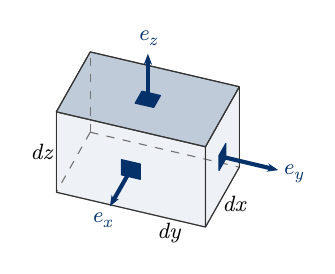
\begin{tikzpicture}[line join=round]
\filldraw[draw=black!45,fill=Paperblue] (0.414,-2.209) -- (2.308,-2.651) -- (2.308,-1.631) -- (0.414,-1.188) -- cycle;
\filldraw[draw=black!45,fill=Paperblue] (2.738,-1.890) -- (2.308,-2.651) -- (2.308,-1.631) -- (2.738,-0.869) -- cycle;
\filldraw[draw=black!70,fill=FAUblue!25] (0.844,-0.427) -- (0.414,-1.188) -- (2.308,-1.631) -- (2.738,-0.869) -- cycle;
\draw[black!55,dashed] (0.844,-1.447) -- (0.414,-2.209);
\draw[black!55,dashed] (0.844,-1.447) -- (2.738,-1.890);
\draw[black!55,dashed] (0.844,-1.447) -- (0.844,-0.427);
\draw[black!80] (0.414,-2.209) -- (2.308,-2.651);
\draw[black!80] (2.308,-2.651) -- (2.738,-1.890);
\draw[black!80] (0.414,-2.209) -- (0.414,-1.188);
\draw[black!80] (2.308,-2.651) -- (2.308,-1.631);
\draw[black!80] (2.738,-1.890) -- (2.738,-0.869);
\draw[black!80] (0.844,-0.427) -- (0.414,-1.188);
\draw[black!80] (0.414,-1.188) -- (2.308,-1.631);
\draw[black!80] (2.308,-1.631) -- (2.738,-0.869);
\draw[black!80] (2.738,-0.869) -- (0.844,-0.427);
\filldraw[draw=FAUblue,fill=FAUblue] (1.242,-1.989) -- (1.480,-2.045) -- (1.480,-1.850) -- (1.242,-1.795) -- cycle;
\draw[-{Stealth[length=4pt]},FAUblue,line width=1.5pt] (1.361,-1.919) -- (1.094,-2.389);
\node[text=FAUblue,fill=white,fill opacity=0.85,text opacity=1,inner sep=1pt,font=\footnotesize] at (0.997,-2.561) {\textit{e\textsubscript{x}}};
\filldraw[draw=FAUblue,fill=FAUblue] (2.567,-1.782) -- (2.480,-1.933) -- (2.480,-1.741) -- (2.567,-1.588) -- cycle;
\draw[-{Stealth[length=4pt]},FAUblue,line width=1.5pt] (2.524,-1.760) -- (3.233,-1.928);
\node[text=FAUblue,fill=white,fill opacity=0.85,text opacity=1,inner sep=1pt,font=\footnotesize] at (3.426,-1.973) {\textit{e\textsubscript{y}}};
\filldraw[draw=FAUblue,fill=FAUblue] (1.501,-0.925) -- (1.415,-1.078) -- (1.651,-1.132) -- (1.737,-0.981) -- cycle;
\draw[-{Stealth[length=4pt]},FAUblue,line width=1.5pt] (1.577,-1.030) -- (1.577,-0.450);
\node[text=FAUblue,fill=white,fill opacity=0.85,text opacity=1,inner sep=1pt,font=\footnotesize] at (1.577,-0.252) {\textit{e\textsubscript{z}}};
\node[,inner sep=1pt,font=\footnotesize] at (1.850,-2.729) {\textit{dy}};
\node[,inner sep=1pt,font=\footnotesize] at (2.679,-2.359) {\textit{dx}};
\node[,inner sep=1pt,font=\footnotesize] at (0.234,-1.698) {\textit{dz}};
\end{tikzpicture}\par\smallskip{\small\raggedright \textbf{The Cartesian volume element.} Each face is a surface on which one coordinate is fixed. Its patch d\textit{A} is the product of the two edges in the face, and its normal is the unit vector of the fixed coordinate.\par}\end{minipage}
\end{center}

\begin{equationcard}{Area elements, Cartesian}
\[ \begin{gathered} {x}\, \text{fixed}:\, \mathrm{d}{A}\, =\, {e}_{\mathrm{x}}\, \mathrm{d}{y}\, \mathrm{d}{z} \\ {y}\, \text{fixed}:\, \mathrm{d}{A}\, =\, {e}_{\mathrm{y}}\, \mathrm{d}{x}\, \mathrm{d}{z} \\ {z}\, \text{fixed}:\, \mathrm{d}{A}\, =\, {e}_{\mathrm{z}}\, \mathrm{d}{x}\, \mathrm{d}{y} \end{gathered} \]
{\small On the opposite face of a box the normal points the other way, for example \ensuremath{-}\textit{e}\textsubscript{x} d\textit{y} d\textit{z}.}
\end{equationcard}

\begin{equationcard}{Area elements, cylindrical}
\[ \begin{gathered} \text{wall},\, {ρ}\, \text{fixed}:\, \mathrm{d}{A}\, =\, {e}_{ρ}\, {ρ}\, \mathrm{d}{φ}\, \mathrm{d}{z} \\ \text{top}\, \text{or}\, \text{base},\, {z}\, \text{fixed}:\, \mathrm{d}{A}\, =\, \pm {e}_{\mathrm{z}}\, {ρ}\, \mathrm{d}{ρ}\, \mathrm{d}{φ} \\ \text{half}-\text{plane},\, {φ}\, \text{fixed}:\, \mathrm{d}{A}\, =\, {e}_{φ}\, \mathrm{d}{ρ}\, \mathrm{d}{z} \end{gathered} \]
{\small Check: the wall of a cylinder of radius \textit{a} and height \textit{h} has area 2π\textit{a h}; each end disk has π\textit{a}\textsuperscript{2}.}
\end{equationcard}

\begin{equationcard}{Area elements, spherical}
\[ \begin{gathered} \text{sphere},\, {r}\, \text{fixed}:\, \mathrm{d}{A}\, =\, {e}_{\mathrm{r}}\, {r}^{2}\, \sin \, {ϑ}\, \mathrm{d}{ϑ}\, \mathrm{d}{φ} \\ \text{cone},\, {ϑ}\, \text{fixed}:\, \mathrm{d}{A}\, =\, {e}_{ϑ}\, {r}\, \sin \, {ϑ}\, \mathrm{d}{r}\, \mathrm{d}{φ} \\ \text{half}-\text{plane},\, {φ}\, \text{fixed}:\, \mathrm{d}{A}\, =\, {e}_{φ}\, {r}\, \mathrm{d}{r}\, \mathrm{d}{ϑ} \end{gathered} \]
{\small Check: $\int_{0}^{2π} $ $\int_{0}^{π} $ \textit{R}\textsuperscript{2} sin \textit{ϑ} d\textit{ϑ} d\textit{φ} = 4π\textit{R}\textsuperscript{2}, the area of a sphere.}
\end{equationcard}
\end{keepsection}

\begin{keepsection}
\Needspace{15\baselineskip}
\section{A.6 Choosing a system, and three common slips}

\Needspace{12\baselineskip}
Pick the system in which the boundary of the problem is a surface where one coordinate is fixed. The integration limits then become constants, and a symmetric field has only one component.

\Needspace{10\baselineskip}
\begin{center}\small\begin{tabularx}{\linewidth}{>{\raggedright\arraybackslash}X>{\raggedright\arraybackslash}X>{\raggedright\arraybackslash}X}\toprule
\textbf{The problem has} & \textbf{Use} & \textbf{Typical example} \\ \midrule
Flat faces, plates, a box & Cartesian & Plate capacitor, a charged slab \\
An axis: wires, coaxial cables, cylinders & Cylindrical & Line charge, coaxial capacitor \\
A centre: point charges, spheres, shells & Spherical & Point charge, charged sphere \\
\bottomrule\end{tabularx}\end{center}

\Needspace{8\baselineskip}
\begin{itemize}
\item \textbf{Forgetting the length factor.} d\textit{V} is \textit{ρ} d\textit{ρ} d\textit{φ} d\textit{z}, not d\textit{ρ} d\textit{φ} d\textit{z}; the sphere’s d\textit{A} carries \textit{r}\textsuperscript{2} sin \textit{ϑ}. Check the units: every d\textit{V} must come out in m\textsuperscript{3} and every d\textit{A} in m\textsuperscript{2}.
\item \textbf{Moving a varying unit vector out of an integral.} \textit{e}\textsubscript{ρ} depends on \textit{φ}, so $\int $ \textit{e}\textsubscript{ρ} d\textit{φ} over a full circle is 0, not 2π\textit{e}\textsubscript{ρ}. Write it in Cartesian unit vectors first (A.3) and integrate the components.
\item \textbf{Mixing up the two angles.} \textit{ϑ} runs only from 0 to π (pole to pole), while \textit{φ} runs from 0 to 2π (once round). A full sphere is not covered by letting both run to 2π.
\end{itemize}
\end{keepsection}


\vfill{\small Personal reference sheet based on the course’s coordinate-system formula collection (Lehrstuhl für Elektromagnetische Felder), rearranged and explained in my own words; the original table and figures are not reproduced. Not an official FAU publication; check details against the current course material. Made by \textbf{Thanate Amornjiraporn (Focus)}.}

\end{document}
